\documentclass[border=1pt]{standalone}

\usepackage{pgfplots}
\pgfplotsset{compat=1.18}

\begin{document}
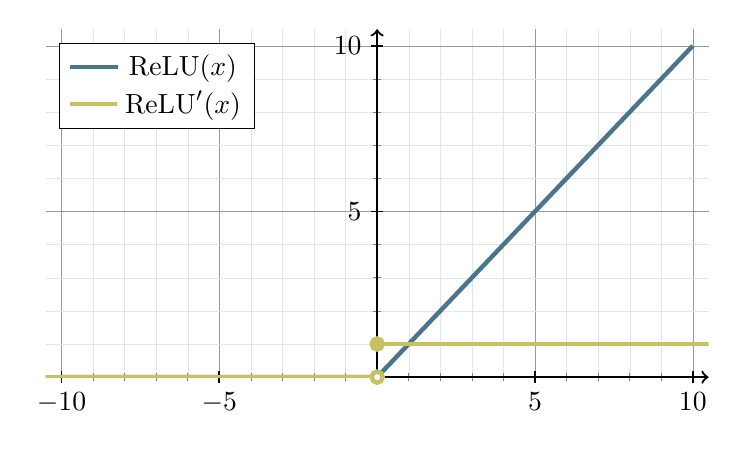
\begin{tikzpicture}
  \begin{axis}[
      scale=1,
      width=10cm,
      height=6cm,
      xmin=-10.5,xmax=10.5,
      ymin=0,ymax=10.5,
      axis x line=center,  axis y line=center,
      minor x tick num=4,
      minor y tick num=4,
      axis line style={-to, thick},
      grid=both,
      grid style={line width=.1pt, draw=gray!20},
      major grid style={line width=.2pt,draw=gray!80},
      xtick={-10, -5,...,10},
      ytick={-10,-5,..., 10},
      every major tick/.style = {
          black, semithick,
        },
      /pgf/number format/.cd, use comma,
      domain=-10:10,
      legend style={at={(0.02,0.96)},anchor=north west}
    ]
    \addplot[ultra thick, cyan!50!black, smooth, samples=250]
    (x,{(x>=0)*x});
    \addlegendimage{ultra thick,yellow!50!gray}
    \addplot[ultra thick, yellow!50!gray, mark=*, samples at={0,11}]
    (x,{1});
    \addplot[ultra thick, yellow!50!gray, mark=*, mark options={fill=white}, samples at={-11,0}]
    (x,{0});
    \legend{$\mathrm{ReLU}(x)$,$\mathrm{ReLU}'(x)$}
  \end{axis}
\end{tikzpicture}
\end{document}
